\documentclass{article}
\title{Bear Grylls Project \\ \large  Using deep reinforcement learning to create an agent able to survive in a hostile environment.}
\author{Erwan Simon}
\usepackage{hyperref}
\usepackage{graphicx}
\usepackage{algorithm2e}
\begin{document}

\maketitle

\tableofcontents

\newpage

\section{Abstract}

\paragraph{•}
We present a world suited to test the capacity of an agent to harvest resources at a minimum speed. It has to navigate around obstacles which interfer with its progression, all of that with limited vision of its environment. An agent enable to maintain a minimal harvesting speed dies.\par
We also provide a description of our tries to implement an algorithm of deep reinforcement learning which can answer to this task in the most efficient way possible.\par

\section{Introduction}

\paragraph{Reinforcement learning}
(RL) is a cutting-edge field in unsupervised learning. Some recent work showed its potential to resolve many complexe problems and beat human expertise in some trivial domains\cite{DBLP:journals/corr/MnihKSGAWR13} and some less trivial ones\cite{healthcare}. The relative earliness of this field may be the cause explaining why it has so much unsolved (or partially solved) problematics among which we can find delayed reward, progression in partially visibe environment (also called non-Markovian decision problem)\cite{bakker2002reinforcement} and generalization to previously unseen situations\cite{sutton1996generalization}.

\paragraph{Deep learning}
has proven to be a good way to improve RL policy (reference needed). Indeed, deep neural networks and their capacities to approximate complexe functions are an excellent tool to represent and perfectionnate the existing links between a state and the result of a action on this state. There is not so much work done in this area relatively speaking compared to other deep learning fields. This could be explain by the fact that reinforcement learning is an ungrateful domain if not deeply uneffective\cite{rlblogpost}. We don't expect here any ground breaking progress considering this paper is more of a domain explorer than a state-of-the-art maker.

\paragraph{The game}
we are presenting here is a solution to test several of the above presented problems. The agent has a limited view of its environment (whence the non-Markovian problem). A reasonably big map paired with random apparition location of the map's features implies that the agent cannot overfit the disposition of its environment, which allow us to test its generalization abilities. Finally, the sparse resources on the map brings the delayed reward problematic. All of this to state that this game is perfect to train deep reinforcement learning agents and test their abilities to survive in hostile environment.

\paragraph{The general hypothesis}
here is that a deep reinforcement learning agent trained with effective parameters can successfully answer the problematics presented above.

\section{Methods}

\subsection{The game}

\subsubsection{The environment}

\paragraph{The board}
is composed by a two-dimensionnal discrete toric world made of squares (technical jargon to say we have a grid where if an agent exists by one side of the board it will come back through the opposit side). A concrete representation can be found in Figure 1.

\begin{figure}
\centering
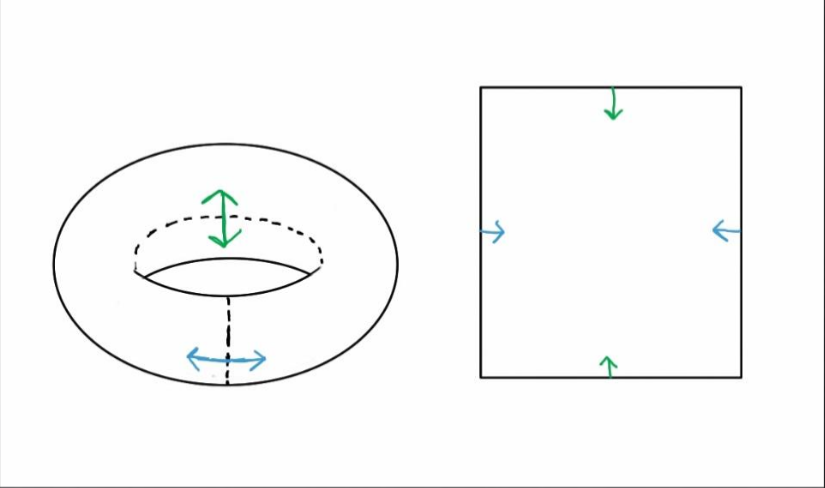
\includegraphics[scale=0.2]{toric_world.png}
\caption{Visual representation of a toric world}
\end{figure}

\paragraph{The food}
appears at random location of the board. They appear as red spot on the map. See figure 2. It grants extra surviving time to agents. The extra time given by one food can be changed to modify the experiment. Raise its value garrantees that agents will have more time before starving to death. If an agent walks on a tile with a food on it, food is transfered to agent inventory and disappears from the tile. Another food then appears in a random location of the board.

\paragraph{Obstacles}
appear at the initial creation of the board and their location never change. They appear as black spot on the map. See figure 2. Percentage of obstacles compared with total number of tile on the board can be set. More obstacles implies more difficulty for an agent to wander around. If an agent try to go on a tile with a trap in it, it just do not move and stays on the tile it was on.

\paragraph{Stones}
spawn at random location on the board. They appear as black spot on the map (smaller than obstacles). See figure 2. If an agent walks on a stone, it picks it and adds it in its inventory. There can be only a limited setable number of stone on the board and in the inventories of agents. Therefore, stones only appears on the board at the begining of the board and when an agent possessing a stone dies. This implies a notion of scarcity of this resource. \par
It does not stricly speaking have any use for an agent to pick a stone yet. Maybe in the future we could imagine a notion of level which could be increased depending on the number of stone possessed by an agent.

\begin{figure}
\centering
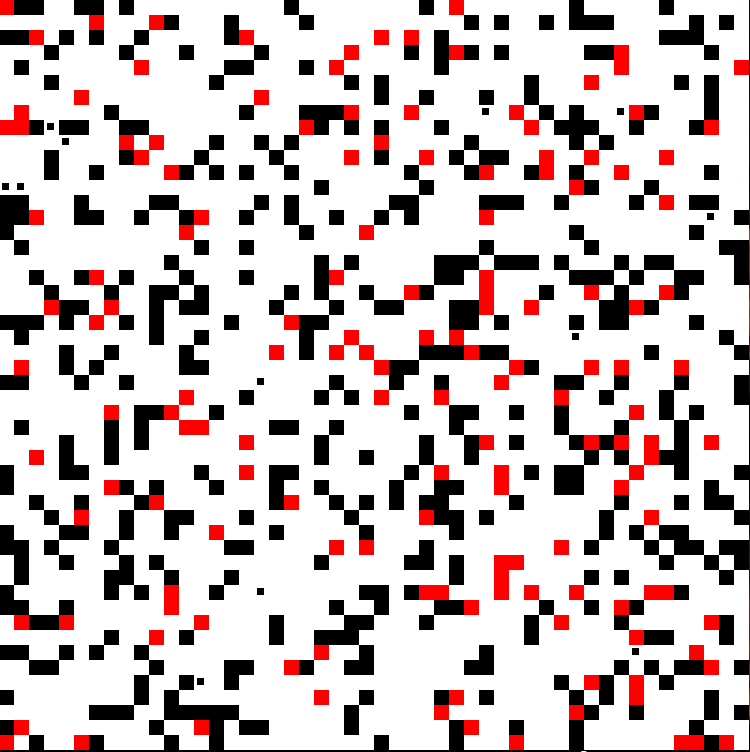
\includegraphics[scale=0.2]{game.png}
\caption{Visual example of the game}
\end{figure}

\subsubsection{The agent}

\paragraph{•}
An agent appears at a random location of the board (location which cannot contain a obstacle) at the begining of the game and when it dies (from starvation). They appear as colored dot surrounded by darker tone area representing its sight. See Figure 3.\par

\paragraph{•}
Inventory of the agents have an amount of food and an amount of stones.

\paragraph{•}
Agents have to move one tile at a time up, down, left or right every turn. They also have a stealing action which if used when in the same tile of another agent which possesses a stone, steals this stone and adds it to the stealer inventory.

\paragraph{•}
Agents have a limited sight of their environment, which wideness is setable. Setting it higher allows them to have a better view on what is around them but it also makes the enviromnent more complexe in their eyes.

\begin{figure}
\centering
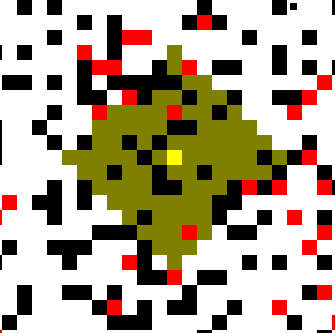
\includegraphics[scale=0.2]{player_example.png}
\caption{Visual example of an agent}
\end{figure}

\subsubsection{The metrics}
The game will be the playground of multiple model from which we need to discriminate the best. To this end I chosed two : the mean number of food possessed by the agent throughout the turns and the mean survival time of an agent throughout the turns. Higher these means are, higher the performance of the agent is.

\subsection{The experiment}

\subsubsection{Reinforcement learning}

Reinforcement learning's different algorithms always have three main parts : the state, the reward and the policy.

\paragraph{The state}
contains the vision of the agent with the surrounding tiles, which allow it to locate food, obstacles and stones. \par
It also contains the current food amount of the agent and the number of stones it possesses. \par
The state is litterally the only mean for the agent to see its surrounding.

\paragraph{The reward}
allows us to say to the agent if something is good or bad. I.E. dying is bad and eating food is good.\par 
Finding the right reward system is very important as well as very difficult. Indeed, a too much explicite one could be considered as cheating because we can no longer consider that the agent discovers the rules of the game by itself. A reward to vague and our agent will not be able to learn anything.\par 
The equilibrium is a vital aspect too. A too punitive reward system could lead to problematic behaviour such as learned helpnessness\cite{wiki:learned_helplessness}. This behaviour leads to unsatisfactory results, like the agent juste going around in circle.\par
It is also very important to not give an either positive nor negative reward if there is not any change in the state, because it encourages the choice of random decisions by the agent (or at least a decision based on wrong inferences). To ensure that it does not happen, I wrote a "rewind algorithm" which stop rewinding when the feature of the map which triggered the reward (food or obstacle) is out of sight. You can see this algorithm in Algorithm 1.\par
Now some events trigger specific rewards. Four do. When the agent just picked a stone, the reward is 1.5. When the agent just ate a food, the reward is 1. When the agent just hitted a wall or died from starvation, the reward is 0 (which is what we call a "negative" reward). Otherwise the reward is set to 0.25. These values will make sens when we will talk about the loss in the deep learning chapter.

\paragraph{The policy}
is the action taken by the agent depending on the current state and the desired state. The main principle of reinforcement learning is to improve the policy tu ensure that the agent will make a decision depending of the state. A good policy improvement eventually ensures that the choice of an action will lead to the maximum possible reward in the medium term (or in the short one).

\paragraph{The bias exploitation-exploration}
is a recurrent dilemna in the reinforcement learning domain. The point is that an agent will learn more and more how to evolve in its environment. We can eventually reach a satisfactory point when the agent can survive in it. But there is always the risk when the agent pleases itself in a sub-optimal behaviour (exploiting) instead of looking for more efficient behaviour (exploring). From a deep learning perspective, it can be seen as a local minimum.\par
To fix this propension by exiting this local minimum, we use a touch of random behaviour until a certain amount of turn. This can be seen as a "training period". With t being the current turn index, we have the condition $random(0, 12500) < 5000 - t$ which if true leads to a random move from the agent. This means that before the 5000th turn, the agent will have a certain chance to act randomly and after 5000 turn, it won't act randomly anymore.

\paragraph{•}
The referencial reinforcement learning algorithms used in this paper are Temporal Difference learning (TD-learning)\cite{tsitsiklis1997analysis} and more precisely Q-Learning\cite{watkins1992q}. The general point of these algorithms are mainly considered as state-of-the-art and more recent ones\cite{mnih2016asynchronous, van2016deep, hessel2018rainbow} only change details which could be considered as minors and unworthy to be detailed here.

\paragraph{•}
Q-learning algorithm being made for Markovian Decision Problem, I had to make a few adjustements to make it compliant with non Markovian Decision problem. Especially the fact that as I said earlier, the reward cannot either positive nor negative if the state doesn't reflect that. The main principle of TD-learning is that when a reward $r$ is given to the agent, you have to rewind to the before rewards to add a portion $r * d$ of the reward $r$. The discount factor $d$ tells the impact of a later reward $r^{t + x}$ on the actual decision process. So the vanilla formula for the reward of TD-learning is :\par
$\forall t' < t$, $r^{t'} = r^{t'} + r^{t' + 1} * d$\par
See the modified algorithm in Algorithm 1.

\begin{algorithm}
\KwIn{$state^t$, $action^t$, $reward^t$, $state^{t+1}$, $dead^t$, $agent$, $discount$, $actions = [UP, RIGHT, DOWN, LEFT]$}
 $reward' = reward^t * discount$\;
 $t' = t$\;
 $actions' = []$\;
 \While{$t'$ != $t + 1$ and $dead^{t'}$ != $True$ and $r' > 1 / len(actions)$ and $len(actions') < player.visionDistance + 1$}{
  \eIf{$(action^{t'} + 2) \% len(actions)$}{
   $actions'.remove((action^{t'} + 2) \% len(actions))$\;
   }{
   $actions'.append(action^{t'})$\;
  }
  $reward^{t'} = reward^{t'} + reward'$\;
  $reward' = reward' * discount$\;
  $t' = t' - 1$\;
 }
 \caption{Custom rewind algorithm}
\end{algorithm}

\subsubsection{Deep learning}

\paragraph{•}
The optimisation of the policy can be made thanks to deep neural networks. Using deep learning paired with Q-learning creates a modified algorithm called Deep Q-Learning (DQN).

\paragraph{•}
I made several tests about which deep neural network architecture was the best suited for this problem.\par
Concerned about the risk of performing worth than randomness, I made an agent which only make random decisions when picking a direction. This way I could say if the performances of a given model were indeed remarquable or not.\par
I started with a simple network with three fully-connected layers with ReLu gave me the first envouraging results, making the agent able to survive a lot more than randomness would. This architecture takes as input the current state $s^t$ of the agent (what is around it, the number of food and stones it possesses and outputs a softmax giving the most appropriate action $a^t$ the agent should take according to the actual policy given by the model. For example, the model could output $a^t = [0.34, 0.11, 0.05, 0.5]$ in which case the agent would go left.\par
Once the model output an action $a^t$, the agent applies it in the game. Therefore the agent is in a new state $s^{t + 1}$ resulting from its action $a^t$ . A new state $s^{t + 1}$ implies a new reward $r^{t + 1}$. This new reward $r^{t + 1}$ tells us whether the action $a^t$ taken with the state $s^t$ was good or bad. A good one should be encouraged and a bad one should be discouraged.\par
To ensure the perpetration of positive behaviour from the agent, I use a loss and an optimizer. I tried many and I chosed to keep the ones that proved to be the most performant, MSE loss and Adam optimizer\par
We calculate the loss by sending to the criterion the same output the model predicted except that we change it a bit. We change the probability of the action taken by the reward extracted from next state. Therefore in the array $a^t$ we change $a^t[argmax(a^t)] = r^{t+1}$ and then send it to the MSELoss as the target along with the regular output $a^t$.

\paragraph{•}
I had an intuition. I knew what I already had was promessing, but it was a really heavy architecture. Each tile of vision contains three pieces of information. Is there a food on this tile ? Is there a stone on this tile ? Is there an obstacle on this tile ? All this information is stored in an one-hot vector, one per tile. The formula to get the number of tile with the agent's sight size $s$ is $s^2 + s * 2$. Add to this the number of stones and the number of food and the number of input neurons $n(s)$ for our fully connected network with a sight size $s$ therefore is $n(s) = (s^2 + s * 2) * 3 + 2$.\par
Imagine now if we raise up the sight distance. For a sight distance $s = 4$ we have $n(4) = 74$ inputs. Now in Figure 3 we have a sight distance of 7, which gives us $n(7) = 191$ inputs. See this is tough complications ahead of our model. I needed a model more robust to inputs augmentation.\par
That is why I immediatly thought about convolutionnal network. It was the perfect answer. More sight distance would not be a problem and would not change the number of parameters. Even adding more information to the state like I did with the stone (initially the stones were not implemented, I added them after) would not add that much parameters, only a feature level.\par
This gives us a new architecture. We have a convolutionnal layer composed of a three dimensionnal filter (stones, food and obstacles) with a max pooling to which we send the vision of the agent. Then we append the number of food and the number of stones to convolutionnal layer output and send it to a fully-connected layer with sigmoïd and softmax which gives us the precognized action.\par
You can see the efficiency of fully-connected network (base) compared to the mixed convolutionnal network (convolutionnal) in Figure 4. We can see the convolutionnal network outperforms the baseline I had.

\begin{figure}
\centering
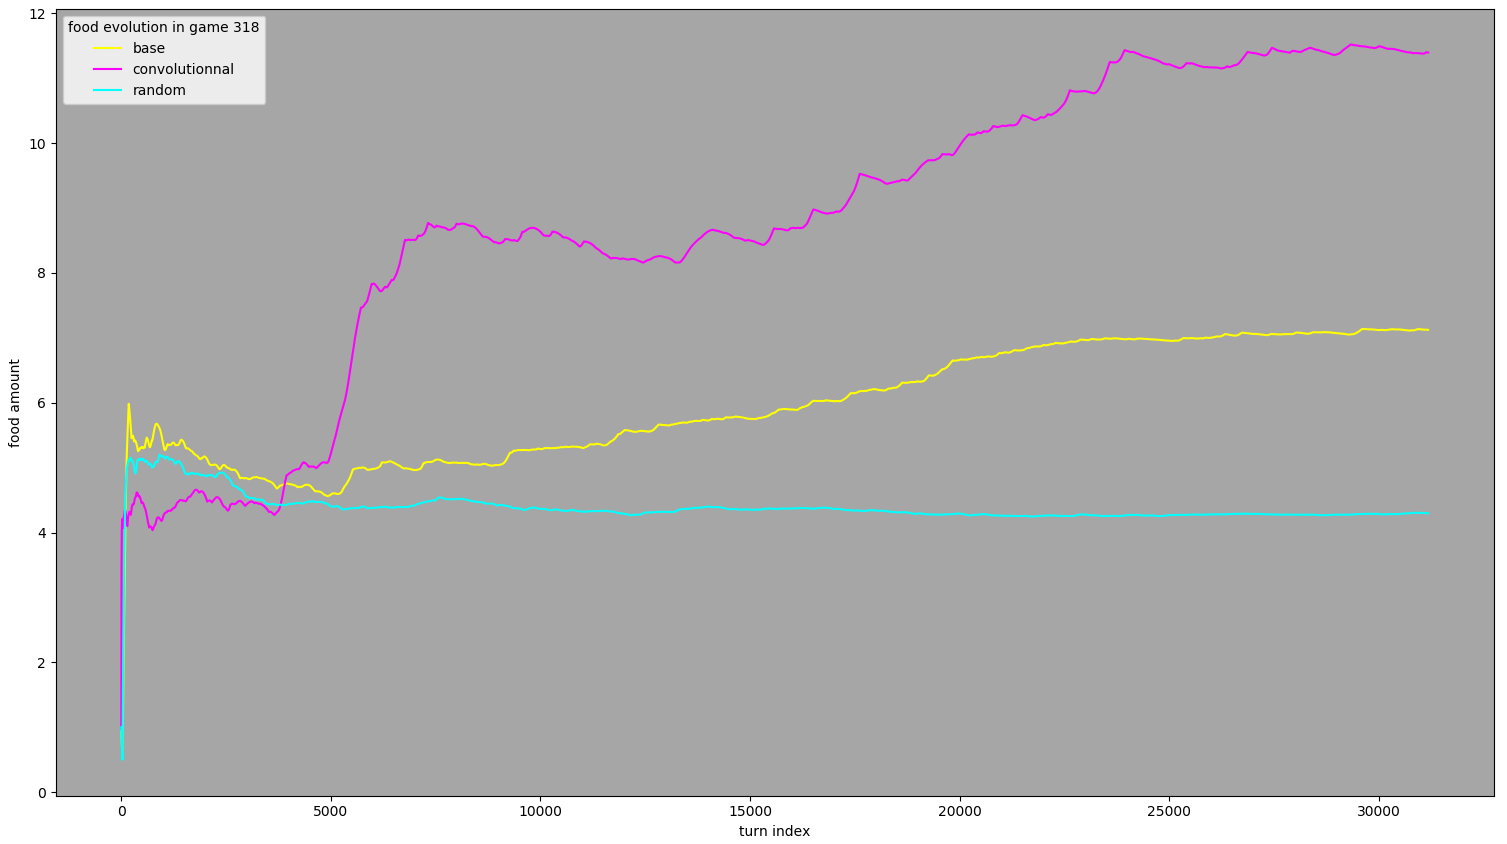
\includegraphics[scale=0.35]{figure_5.png}
\caption{Performance comparaison between models}
\end{figure}

\paragraph{•}
Everytime the agent dies, we pick randomly some state from its memory and we pass it through the model to train it on some already seen scenarios. We don't send every elements of its memory otherwise the training after each death quicly lasts a consequent time. We fixed the "batch size" to 20 000 elements.\par
I talked about learned helpnessness\cite{wiki:learned_helplessness} earlier. Now to prevent such things from happening, I figured out that it was better if instead of picking fully randomly elements of the agent memory, we were picking the same amount of situation where the agent :\par
- died or hit an obstacle;\par
- ate food or a stone;\par
- did nothing remarquable at all (to show the model examples of neutral behaviour to "normalize" it).\par

\section{Results}

\paragraph{•}
The game seems to offer some concrete possibilities to test effectively and without bias deep reinforcement learning models.

\paragraph{•}
The result I obtained were promessing. A little finetuning made me obtained good results as I could see agents going around obstacles to pick food, aquirering such a rythm in its food harvesting that it eventually stopped starving to death. Which was, if I could put it like that, the purpose of the experiment, an autonomous agent surviving in a hostile environment.

\paragraph{•}
Some odd situations kept happening though. I regretfully notted that sometimes, the agent suddenly start to go around in circle. This even can occures after seeing the same agent perform extremly well. The agent seems to have reached a sort of local minimum from where it cannot reach out.

\paragraph{•}
I also surprisingly notted that adding complexity to models did not allow to gain in performance and sometimes led to the exact contrary. One point for the Ockam Razor.

\section{Discussion}

\paragraph{The dimensionnal aspect}
from the problem brought to me another intuition. The most suited model to handle temporal problems might be recurrent neural networks (RNN). Some wrote about using RNN in reinformement learning problems\cite{bakker2002reinforcement} but I did not have time to successfully apply their methods.

\paragraph{•}
One lead could also be promessing in my opinion. I found that the performances of an agent were drastically dropping after the "training session", when it stopped using random action. Ths can be explain by the fact the agent can sometimes be saved by a random action if it is stuck in a tough spot of the map.\par
To fix this I thought about two things. Either make the agent have a certain amount of randomness forever (a little bit of constant exploring). Either make that if suddenly the performance of the agent drop, it starts a "new train session" and start to pick random action all over again.

\paragraph{•}
The source code is publicly available on my github\cite{github:bear_grylls_project}.


\bibliographystyle{unsrt}
\bibliography{sources}

\end{document}